\documentclass[11pt,a4paper]{article}
\usepackage[T1]{fontenc}
\usepackage[utf8]{inputenc}
\usepackage{mathpazo}
\usepackage{courier}
\usepackage[margin=2.5cm]{geometry}
\usepackage{graphicx}
\usepackage{booktabs}
\usepackage{float}
\usepackage{array}
\usepackage{microtype}
\usepackage[font=small,labelfont=bf]{caption}
\usepackage{enumitem}
\usepackage[hidelinks]{hyperref}
\usepackage{url}
\setlength{\parskip}{0.5em}
\setlength{\parindent}{0pt}
\linespread{1.05}
\setlist{itemsep=0.2em,topsep=0.3em}
\newcommand{\ra}{$\rightarrow$}
\hypersetup{pdftitle={Is It the Encoder or the Head? Slide-Level Robustness of Pathology Foundation Models on CAMELYON16},pdfauthor={Dinakar Pathakota}}

\title{\textbf{Is It the Encoder or the Head?\\ Slide-Level Robustness of Pathology Foundation Models\\ to Acquisition Artifacts on CAMELYON16}}
\author{Dinakar Pathakota\\[0.3em]
\small Independent Researcher, Hyderabad, India\\
\small \texttt{dinakar.pathakota@gmail.com}}
\date{12 October 2026\\[0.3em]\small Technical report, version 1}

\begin{document}
\maketitle

\begin{abstract}
\noindent A previous report found that much of the accuracy a frozen pathology foundation model loses under image degradation belongs to the linear probe on top, not to the encoder. That study used patch classification. Here we ask the same question for slide-level detection of lymph-node metastases on CAMELYON16 (399 whole-slide images, 871,867 tiles at about 10x), with four frozen encoders, seven test conditions and five seeds. With an attention-based multiple-instance head, training on a mix of clean and degraded tile embeddings recovers much of the loss to JPEG compression for Phikon and Kaiko B/16: at quality 10, which the head never saw, slide AUC rises from 63.1 to 79.7 and from 67.9 to 81.1, with no change on clean slides. It does not help Phikon-v2. Three analyses show the tumour signal survives in the encoder where the attention head fails: for the three pathology encoders, a linear probe on single tiles trained on mixed tiles still separates tumour at a tile AUC of 92 to 98 under JPEG quality 10 and blur $\sigma$ 4; mixed training moves Phikon-v2's attention away from tumour; and a slide head built from tile-level supervision does recover with mixed training, reaching 69.6 to 70.8 AUC under blur where attention stays at 54 to 60. Pooled AUC also hides what matters clinically. At 95\% specificity, Phikon's attention head detects 96\% of tumour slides on clean images; under JPEG quality 10 it detects 37\% when trained on clean embeddings and 60\% when trained on mixed ones, and the loss falls on small metastases. Under heavy blur, the clean-trained attention scores of two of the encoders separate the two hospitals almost perfectly. We recommend reporting slide-level robustness by tumour size, at a fixed operating point and within each centre. Code and results: \url{https://github.com/dinakar0745/camelyon-slide-study}.
\end{abstract}

\section{Introduction}

Pathology foundation models are used as frozen tile encoders, and most clinical tasks are decided at the level of the whole slide. A slide is cut into thousands of tiles, each tile is embedded, and a small aggregation head turns the bag of embeddings into one prediction. Whether this pipeline stays accurate when image quality drops is a practical question: scanners produce out-of-focus regions, archives are compressed, and staining varies.

In an earlier report we studied this at patch level (Pathakota, 2026). With the encoder frozen, a linear probe trained on a mix of clean and degraded embeddings recovered most of the accuracy that a clean-trained probe lost to compression and stain shift. The information was still in the embeddings; the clean-trained probe read them along the wrong direction. That study left out slide-level aggregation, which is where the clinical decision is made, and where a few tumour tiles must stand out among thousands of normal ones.

This report asks the same question at slide level, on lymph-node metastasis detection in CAMELYON16 (Ehteshami Bejnordi et al., 2017). We keep four frozen encoders and train slide-level heads on clean or on mixed tile embeddings, then test them on all 129 test slides under seven conditions. Our contributions are:

\begin{enumerate}
\item \textbf{Mixed training helps at slide level, but not for every encoder.} For an attention-based multiple-instance head, mixed training recovers 12 to 17 AUC points under JPEG quality 15 and 10 for Phikon and Kaiko B/16 at no cost on clean slides. It gives nothing for Phikon-v2, which at patch level gained the most from mixed training at JPEG quality 10 on NCT-CRC-HE.
\item \textbf{Where the attention head fails, the encoder still carries the signal.} Tile-level probes separate tumour under every degradation we tested when trained on mixed tiles, and a slide head built from tile-level supervision recovers under JPEG and blur where the attention head does not. For Phikon-v2, mixed training moves attention away from tumour.
\item \textbf{Pooled AUC hides the clinically relevant loss.} At 95\% specificity, degradation removes the detection of small metastases first, while most slides with more than 200 tumour tiles are still found under compression.
\item \textbf{Degradation interacts with the hospital.} Under heavy blur, the clean-trained attention scores of Phikon and Phikon-v2 become close to a hospital detector. Within-centre analysis shows effects that the pooled number hides.
\end{enumerate}

As in the first report, the mixed head is not proposed as a method. It is a baseline that separates what the encoder lost from what the head failed to use.

\section{Related work}

\textbf{Patch-level robustness.} Yajnik et al.\ (2026) benchmark 12 pathology foundation models under optimised perturbations with clean-trained linear probes on patch tasks. Our first report added the probe as an experimental variable and found that a degradation-aware probe recovers most losses to compression and stain shift (Pathakota, 2026). Hasan et al.\ (2026) measure embedding drift under JPEG2000 without downstream accuracy.

\textbf{Centre effects.} De Jong et al.\ (2025) and K\"omen et al.\ (2026) show that foundation-model features encode the medical centre, and K\"omen et al.\ report that slide-level tumour detection on Camelyon collapses towards chance when centre and label are confounded in training. We do not confound training data; we find that synthetic degradation makes slide scores track the centre on unconfounded data.

\textbf{Slide-level aggregation.} Attention-based multiple-instance learning (Ilse et al., 2018) is the standard head on frozen tile embeddings. Campanella et al.\ (2019) trained slide classifiers from slide labels alone with a max-pooling instance classifier. We compare an attention head trained on slide labels with a head that uses tile labels from the lesion annotations, to locate where degraded signal is lost; we do not propose either.

\section{Method}

\subsection{Data}

CAMELYON16 contains 399 haematoxylin and eosin stained sentinel lymph-node slides from two Dutch centres, Radboud University Medical Center (RUMC) and University Medical Center Utrecht (UMCU), with lesion-level annotations of every metastasis in tumour slides (Ehteshami Bejnordi et al., 2017; Litjens et al., 2018). We use the official split (Table~\ref{tab:data}) and the public copy on the Registry of Open Data on AWS. The centre of each slide is read from its pixel spacing (0.243 microns per pixel for RUMC, about 0.226 for UMCU). Test tumour slides are labelled macro- or micrometastasis in the official reference file.

\begin{table}[h]\centering\small
\caption{Slides used. Tumour tiles are tiles with any annotated tumour.}
\label{tab:data}
\begin{tabular}{@{}lccc@{}}
\toprule
 & Slides & RUMC / UMCU & Median tumour tiles per tumour slide\\
\midrule
Training, normal & 159 & 100 / 59 & \\
Training, tumour & 111 & 71 / 40 & 58\\
Test, normal & 80 & 50 / 30 & \\
Test, macrometastasis & 22 & 13 / 9 & 272\\
Test, micrometastasis & 27 & 11 / 16 & 10\\
\bottomrule
\end{tabular}
\end{table}

\textbf{Tiling.} Each slide is read at a downsample of 4 from full resolution, 0.91 to 0.97 microns per pixel (roughly 10x), and cut into non-overlapping $224 \times 224$ pixel tiles on a grid anchored at the slide origin. Tissue is found by Otsu thresholding of saturation on a 1/32 overview, and tiles with at least 25\% tissue are kept: 871,867 tiles in all, a median of 1,945 per training slide and 1,826 per test slide. The lesion annotations are rasterised at the same 1/32 scale, with exclusion regions removed, to give the tumour fraction of every tile.

\subsection{Encoders and degradations}

We use the four encoders of the first report, frozen, with their published preprocessing: Phikon (ViT-B/16; Filiot et al., 2023), Phikon-v2 (ViT-L/16; Filiot et al., 2024), Kaiko B/16 (ViT-B/16; Aben et al., 2024) and the natural-image DINOv2-L (ViT-L/14; Oquab et al., 2023). Each tile is represented by the CLS embedding, computed in 32-bit precision and stored as 16-bit floats. No CAMELYON16 slide appears in the published pretraining data of any encoder; the Phikon-v2 authors use Camelyon16 as an external test set.

Degradations are applied to each tile at 10x, before the encoder's preprocessing, with the functions of the first report: Gaussian blur ($\sigma$ in pixels), JPEG compression (quality factor) and stain shift (haematoxylin scaled by $1+\alpha$, eosin by $1-\alpha$). Test slides are embedded under seven conditions: clean, blur $\sigma$ 2 and 4, JPEG quality 30, 15 and 10, and stain $\alpha$ 0.3. Training slides are embedded clean and once as \emph{mixed}: each tile is drawn at random from clean, blur $\sigma$ 2 and 4, JPEG quality 30 and 15, and stain $\alpha$ 0.3, with the draw fixed per tile. JPEG quality 10 is therefore never seen in training, and both training sets have the same tiles.

\subsection{Slide-level heads}

All heads standardise tile embeddings with the mean and standard deviation of the tiles of the slides they are fitted on.

\begin{itemize}
\item \textbf{Mean and max pooling:} logistic regression on the mean, or the per-dimension maximum, of a slide's tile embeddings. The regularisation $C$ is chosen from $10^{-4}$ to 10 by validation AUC.
\item \textbf{Attention MIL:} gated attention-based multiple-instance learning (Ilse et al., 2018) with a 256-unit tile projection, 128-unit attention, dropout 0.25, Adam (learning rate $10^{-4}$, weight decay $10^{-4}$), one slide per step, 40 epochs. The epoch with the best validation AUC is kept. It sees slide labels only.
\item \textbf{Tile head:} logistic regression ($C = 1$, balanced class weights) on single tiles, trained on tiles at least half tumour from tumour slides and a random 30,000 tiles from normal slides. A slide's score is the mean of its $k$ highest tile scores, with $k$ chosen from 1 to 50 by validation AUC. It uses the lesion annotations, which the other heads do not.
\end{itemize}

Each head is trained with five seeds. Each seed fits on a stratified random 80\% of the 270 training slides and makes its one choice ($C$, epoch or $k$) on the other 20\%. The split depends only on the seed, so the clean- and mixed-trained heads of a seed are compared on the same slides. The test set is used only for the final scores. The settings of the mean, max and attention heads were fixed before any test result was seen. The tile head and the analyses in Sections~\ref{sec:encoder} to~\ref{sec:hospital} were designed after the first results, to explain them.

\subsection{Metrics and analyses}

\textbf{Slide AUC.} We report the mean and standard deviation over seeds of the AUC on all 129 test slides, and on macro- and micrometastasis slides each against all 80 normal slides. Intervals are 95\% stratified bootstrap intervals over test slides (2,000 resamples) of the mean over seeds. The gain from mixed training is paired by seed and by resample.

\textbf{Operating point.} Sensitivity at 95\% specificity uses, for each seed, the threshold that lets 4 of the 80 normal test slides through. It is reported overall and by the number of tiles touching tumour.

\textbf{Attention.} For attention heads, on each test tumour slide we record whether the most-attended tile touches tumour. Changes from mixed training are averaged over seeds per slide and bootstrapped over slides.

\textbf{Drift and tile probes.} Drift is the cosine similarity between a tile's degraded and clean embedding, in the clean-standardised space. The tile probe is the tile-level classifier of the tile head trained on all 270 training slides, tested on test tiles that are at least half tumour against all tiles of the 80 normal test slides.

\textbf{Centre.} AUC is computed within each centre, and we measure how well a head's score tells the centres apart among normal test slides (AUC of the score for UMCU against RUMC; 50 means not at all).

\subsection{Software and compute}

Slides were tiled with tiffslide 4.0.0 (tifffile 2026.9.20, imagecodecs 2026.8.16). Embeddings, heads and analyses used the software of the first report: PyTorch 2.11.0 (CUDA 12.8), transformers 5.18.0, timm 1.0.30 with torchvision 0.26.0, Pillow 12.3.0, scikit-image 0.26.0, scikit-learn 1.9.1, NumPy 2.5.3 and SciPy 1.18.1 on Python 3.14.8 under Windows, on one NVIDIA RTX 3050 laptop GPU with 4 GB. Slides were downloaded, tiled and deleted one at a time so that the project stayed under 50 GB of disk; the 701 GB of slides were never held at once. Training the mean, max and attention heads for all encoders took 58 minutes. Refitting the attention heads for the analyses reproduced the committed clean test AUC to the first decimal for every encoder and training set.

\section{Results}

\subsection{Aggregation decides clean accuracy}

On clean slides, the head matters more than the encoder (Table~\ref{tab:heads}). Mean pooling reaches only 59.2 to 66.5 AUC and max pooling 61.3 to 79.4, because a tumour slide has a median of 50 tumour tiles among about 2,000. Attention MIL reaches 98.9 (Phikon), 98.6 (Kaiko) and 96.4 (Phikon-v2). DINOv2-L stays at 77.3 with attention and 78.8 with the tile head. We report attention MIL and the tile head from here on; the pooled heads are in the appendix.

\begin{table}[h]\centering\small
\caption{Clean test slides, heads trained on clean embeddings. Slide AUC in \%, mean $\pm$ standard deviation over five seeds.}
\label{tab:heads}
\begin{tabular}{@{}lcccc@{}}
\toprule
Head (clean-trained) & Phikon & Kaiko B/16 & Phikon-v2 & DINOv2-L\\
\midrule
Mean pooling & 66.5{\scriptsize$\pm$3.1} & 64.3{\scriptsize$\pm$2.3} & 61.3{\scriptsize$\pm$3.8} & 59.2{\scriptsize$\pm$0.6}\\
Max pooling & 79.4{\scriptsize$\pm$1.6} & 77.1{\scriptsize$\pm$2.2} & 75.4{\scriptsize$\pm$1.3} & 61.3{\scriptsize$\pm$2.7}\\
Attention MIL & 98.9{\scriptsize$\pm$0.4} & 98.6{\scriptsize$\pm$0.4} & 96.4{\scriptsize$\pm$1.5} & 77.3{\scriptsize$\pm$2.8}\\
Tile head & 92.7{\scriptsize$\pm$1.2} & 91.1{\scriptsize$\pm$1.6} & 93.0{\scriptsize$\pm$2.8} & 78.8{\scriptsize$\pm$1.9}\\
\bottomrule
\end{tabular}
\end{table}

\subsection{Mixed training at slide level}

Table~\ref{tab:main} and Figure~\ref{fig:auc} compare heads trained on clean and on mixed embeddings. With attention MIL, mixed training raises Phikon from 74.0 to 86.2 at JPEG quality 15 (gain 12.2, interval 5.9 to 18.8) and from 63.1 to 79.7 at quality 10 (16.7, 9.1 to 24.1). Kaiko rises from 75.3 to 89.7 and from 67.9 to 81.1. Clean AUC changes by $-0.1$ for both. The gains are largest on micrometastases: 20.7 points for Phikon at quality 10 and 22.1 for Kaiko at quality 15 (Table~\ref{tab:gains}).

Phikon-v2 is the exception. Mixed training changes its attention head by $-0.3$ at JPEG quality 10 and $+2.3$ at quality 15, with intervals spanning zero, and lowers clean AUC from 96.4 to 93.8 (gain $-2.6$, interval $-5.7$ to $-0.1$). In the first report, at patch level on NCT-CRC-HE at JPEG quality 10, Phikon-v2 gained the most of any encoder (balanced accuracy from 49.1 to 88.1).

Blur $\sigma$ 4 brings every attention head close to chance (51.0 to 56.2), and mixed training leaves it there (53.9 to 60.0), although $\sigma$ 4 was in the mixed training set. Stain shift at $\alpha$ 0.3 costs nothing.

\begin{table}[h]\centering\small
\caption{Slide AUC in \%, all 129 test slides, mean of five seeds: head trained on clean embeddings \ra{} head trained on mixed embeddings. JPEG Q10 was not in the mixed training set.}
\label{tab:main}
\begin{tabular}{@{}lcccc@{}}
\toprule
Condition & Phikon & Kaiko B/16 & Phikon-v2 & DINOv2-L\\
\midrule
\multicolumn{5}{@{}l}{\textit{Attention MIL}}\\
Clean & 98.9 \ra{} 98.8 & 98.6 \ra{} 98.5 & 96.4 \ra{} 93.8 & 77.3 \ra{} 76.4\\
Blur $\sigma$ 2 & 90.1 \ra{} 95.5 & 97.6 \ra{} 97.9 & 86.1 \ra{} 87.5 & 71.0 \ra{} 71.7\\
Blur $\sigma$ 4 & 51.0 \ra{} 53.9 & 55.6 \ra{} 60.0 & 56.2 \ra{} 54.8 & 53.0 \ra{} 58.9\\
JPEG Q30 & 90.4 \ra{} 92.3 & 93.6 \ra{} 96.7 & 84.6 \ra{} 85.7 & 72.0 \ra{} 76.3\\
JPEG Q15 & 74.0 \ra{} 86.2 & 75.3 \ra{} 89.7 & 72.7 \ra{} 75.0 & 70.5 \ra{} 74.6\\
JPEG Q10 (unseen) & 63.1 \ra{} 79.7 & 67.9 \ra{} 81.1 & 68.1 \ra{} 67.8 & 70.0 \ra{} 74.4\\
Stain $\alpha$ 0.3 & 99.4 \ra{} 99.2 & 98.5 \ra{} 98.2 & 97.2 \ra{} 94.5 & 77.9 \ra{} 78.4\\
\addlinespace
\multicolumn{5}{@{}l}{\textit{Tile head}}\\
Clean & 92.7 \ra{} 89.9 & 91.1 \ra{} 90.0 & 93.0 \ra{} 87.5 & 78.8 \ra{} 75.0\\
Blur $\sigma$ 2 & 73.2 \ra{} 86.5 & 83.4 \ra{} 88.9 & 77.8 \ra{} 82.8 & 72.3 \ra{} 72.6\\
Blur $\sigma$ 4 & 59.3 \ra{} 69.8 & 52.4 \ra{} 70.8 & 58.0 \ra{} 69.6 & 53.9 \ra{} 59.0\\
JPEG Q30 & 84.5 \ra{} 90.2 & 90.9 \ra{} 91.2 & 84.3 \ra{} 86.2 & 78.0 \ra{} 75.8\\
JPEG Q15 & 74.4 \ra{} 87.9 & 87.5 \ra{} 89.3 & 77.7 \ra{} 85.1 & 78.2 \ra{} 76.8\\
JPEG Q10 (unseen) & 71.0 \ra{} 88.2 & 82.1 \ra{} 89.6 & 75.8 \ra{} 81.9 & 77.6 \ra{} 77.3\\
Stain $\alpha$ 0.3 & 91.4 \ra{} 91.9 & 91.9 \ra{} 89.4 & 93.1 \ra{} 88.6 & 79.8 \ra{} 80.4\\
\bottomrule
\end{tabular}
\end{table}

\begin{figure}[t]\centering
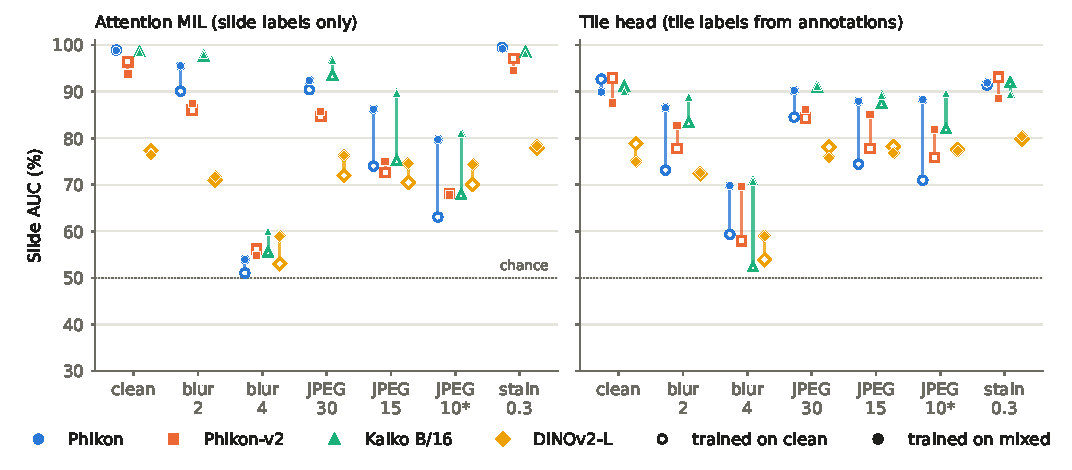
\includegraphics[width=\linewidth]{fig1_slide_auc.pdf}
\caption{Slide AUC on the 129 test slides under each condition, for heads trained on clean embeddings (hollow) and mixed embeddings (filled), mean of five seeds. Left: attention MIL, trained from slide labels. Right: tile head, trained from tile labels. *JPEG quality 10 was not in the mixed training set.}
\label{fig:auc}
\end{figure}

\subsection{Is it the encoder or the head?}
\label{sec:encoder}

Three measurements locate the loss (Table~\ref{tab:enchead}).

\textbf{Drift.} Phikon-v2's embeddings move furthest under compression. At JPEG quality 10, the cosine similarity between a tumour tile's degraded and clean embedding is 0.17 for Phikon-v2, against 0.28 for Phikon and 0.30 for Kaiko.

\textbf{The signal survives in the encoder.} A tile probe trained on clean tiles still separates tumour tiles from normal-slide tiles at a tile AUC of 94.1 for Phikon-v2 at JPEG quality 10, higher than Phikon's 81.1. Trained on mixed tiles, the probe reaches 96.9 to 98.4 for the three pathology encoders at quality 10, and 92.2 to 93.8 at blur $\sigma$ 4.

\textbf{The attention head loses it.} At JPEG quality 10, mixed training makes the most-attended tile land on tumour more often for Phikon (by 15.1 points of slides) and Kaiko (9.8), and less often for Phikon-v2 ($-6.9$, interval $-11.4$ to $-2.9$). At blur $\sigma$ 4, mixed training moves attention away from tumour for Phikon ($-11.4$) and Kaiko ($-10.2$), and the change for Phikon-v2 ($-6.9$) has an interval spanning zero.

\textbf{A head with tile supervision recovers.} The tile head, trained on mixed tiles, reaches 88.2 (Phikon), 89.6 (Kaiko) and 81.9 (Phikon-v2) at JPEG quality 10, against 79.7, 81.1 and 67.8 for mixed-trained attention, and 69.6 to 70.8 at blur $\sigma$ 4 against 53.9 to 60.0. For Phikon-v2, mixed training now helps: by 7.3 points at JPEG quality 15 (interval 1.3 to 13.3) and 11.6 at blur $\sigma$ 4 (0.8 to 22.2). Under blur, the recovery is in large metastases: on macrometastasis slides mixed training gains the tile head 20.8 to 30.2 points for the three pathology encoders, while on micrometastases the change is not distinguishable from zero for any encoder (Table~\ref{tab:gains}).

So for compression, and for large metastases under blur, the tumour signal is still in the frozen embeddings. The attention head, which learns only from slide labels, does not find it under blur for any encoder, nor under compression for Phikon-v2, whose degraded tumour tiles move furthest from their clean position; given tile labels, a linear head recovers in both cases. The tile head pays for this on clean slides: mixed training costs it 1.2 to 5.4 points there, mostly on micrometastases.

\begin{table}[h]\centering\small
\caption{Encoder or head, at JPEG Q10 and blur $\sigma$ 4. Cosine: mean over tumour tiles of test tumour slides. Tile probe: tile AUC in \%. Top-attended tile: \% of the 49 test tumour slides whose most-attended tile touches tumour, mean of five seeds; the change from mixed training is averaged per slide with a 95\% bootstrap interval over slides (bold: excludes zero). Slide AUC in \%.}
\label{tab:enchead}
\setlength{\tabcolsep}{4pt}
\resizebox{\linewidth}{!}{\begin{tabular}{@{}lcccc@{}}
\toprule
 & Phikon & Kaiko B/16 & Phikon-v2 & DINOv2-L\\
\midrule
\multicolumn{5}{@{}l}{\textit{JPEG Q10 (unseen)}}\\
Cosine to clean, tumour tiles & 0.28 & 0.30 & 0.17 & 0.36\\
Tile probe, tile AUC (clean \ra{} mixed) & 81.1 \ra{} 97.2 & 94.9 \ra{} 98.4 & 94.1 \ra{} 96.9 & 90.4 \ra{} 95.6\\
Top-attended tile on tumour, \% (clean \ra{} mixed) & 48.6 \ra{} 63.7 & 60.8 \ra{} 70.6 & 42.4 \ra{} 35.5 & 49.0 \ra{} 53.5\\
\quad change from mixed training & \textbf{+15.1 {\scriptsize[+7.3, +23.7]}} & \textbf{+9.8 {\scriptsize[+3.7, +16.7]}} & \textbf{-6.9 {\scriptsize[-11.4, -2.9]}} & \textbf{+4.5 {\scriptsize[+0.8, +8.2]}}\\
Slide AUC, mixed-trained: attention / tile head & 79.7 / 88.2 & 81.1 / 89.6 & 67.8 / 81.9 & 74.4 / 77.3\\
\addlinespace
\multicolumn{5}{@{}l}{\textit{Blur $\sigma$ 4}}\\
Cosine to clean, tumour tiles & 0.22 & 0.23 & 0.21 & 0.03\\
Tile probe, tile AUC (clean \ra{} mixed) & 72.6 \ra{} 93.8 & 63.1 \ra{} 93.2 & 79.9 \ra{} 92.2 & 64.9 \ra{} 87.2\\
Top-attended tile on tumour, \% (clean \ra{} mixed) & 38.8 \ra{} 27.3 & 38.0 \ra{} 27.8 & 35.1 \ra{} 28.2 & 22.4 \ra{} 20.0\\
\quad change from mixed training & \textbf{-11.4 {\scriptsize[-17.6, -5.7]}} & \textbf{-10.2 {\scriptsize[-16.7, -4.5]}} & -6.9 {\scriptsize[-14.3, +0.4]} & -2.4 {\scriptsize[-6.9, +1.6]}\\
Slide AUC, mixed-trained: attention / tile head & 53.9 / 69.8 & 60.0 / 70.8 & 54.8 / 69.6 & 58.9 / 59.0\\
\bottomrule
\end{tabular}}
\end{table}

\subsection{What the AUC hides}
\label{sec:size}

A screening tool runs at one threshold. At 95\% specificity (Table~\ref{tab:sens}), Phikon's clean-trained attention head detects 96\% of the 49 tumour slides on clean images, 49\% at JPEG quality 15, 37\% at quality 10 and 21\% at blur $\sigma$ 4. Mixed training raises the quality 10 figure to 60\%; the mixed-trained tile head reaches 61\% there and 44\% under blur. An AUC near 80 thus means missing about four tumour slides in ten at this operating point.

The loss falls on small metastases (Figure~\ref{fig:size}). On clean images, 10x is not the limit: Phikon's attention head detects 93\% of the 14 slides whose tumour touches only 1 to 10 tiles. At JPEG quality 10 it detects 14\% of them with clean training and 41\% with mixed training. Mixed training recovers mid-sized metastases best: for Phikon's tile head at quality 10, slides with 11 to 50 tumour tiles go from 18\% to 45\% and slides with 51 to 200 from 53\% to 84\%. Large metastases survive compression: attention heads still detect 68 to 100\% of slides with more than 200 tumour tiles under JPEG quality 15 and 10. No head detects more than 23\% of the smallest metastases under blur.

The two heads miss different slides. On clean images, the mixed-trained attention head detects 9 to 11 tumour slides that the mixed-trained tile head misses (Phikon, Kaiko), and the tile head none that attention misses. Under JPEG quality 10 and blur $\sigma$ 4 this reverses: the tile head detects up to 15 slides that attention misses (Phikon-v2 under blur). Slides missed by both are mostly micrometastases.

\begin{table}[h]\centering\small
\caption{Sensitivity in \% at 95\% specificity on the 129 test slides, mean of five seeds.}
\label{tab:sens}
\begin{tabular}{@{}llcccc@{}}
\toprule
Encoder & Head & Clean & JPEG Q15 & JPEG Q10 (unseen) & Blur $\sigma$ 4\\
\midrule
Phikon & Attention, clean-trained & 96 & 49 & 37 & 21\\
 & Attention, mixed-trained & 95 & 73 & 60 & 27\\
 & Tile head, clean-trained & 76 & 52 & 44 & 13\\
 & Tile head, mixed-trained & 74 & 68 & 61 & 44\\
\addlinespace
Phikon-v2 & Attention, clean-trained & 86 & 44 & 31 & 16\\
 & Attention, mixed-trained & 80 & 51 & 37 & 22\\
 & Tile head, clean-trained & 83 & 42 & 40 & 13\\
 & Tile head, mixed-trained & 76 & 63 & 56 & 46\\
\addlinespace
Kaiko B/16 & Attention, clean-trained & 93 & 55 & 45 & 28\\
 & Attention, mixed-trained & 92 & 73 & 57 & 31\\
 & Tile head, clean-trained & 79 & 66 & 49 & 11\\
 & Tile head, mixed-trained & 73 & 74 & 69 & 47\\
\bottomrule
\end{tabular}
\end{table}

\begin{figure}[t]\centering
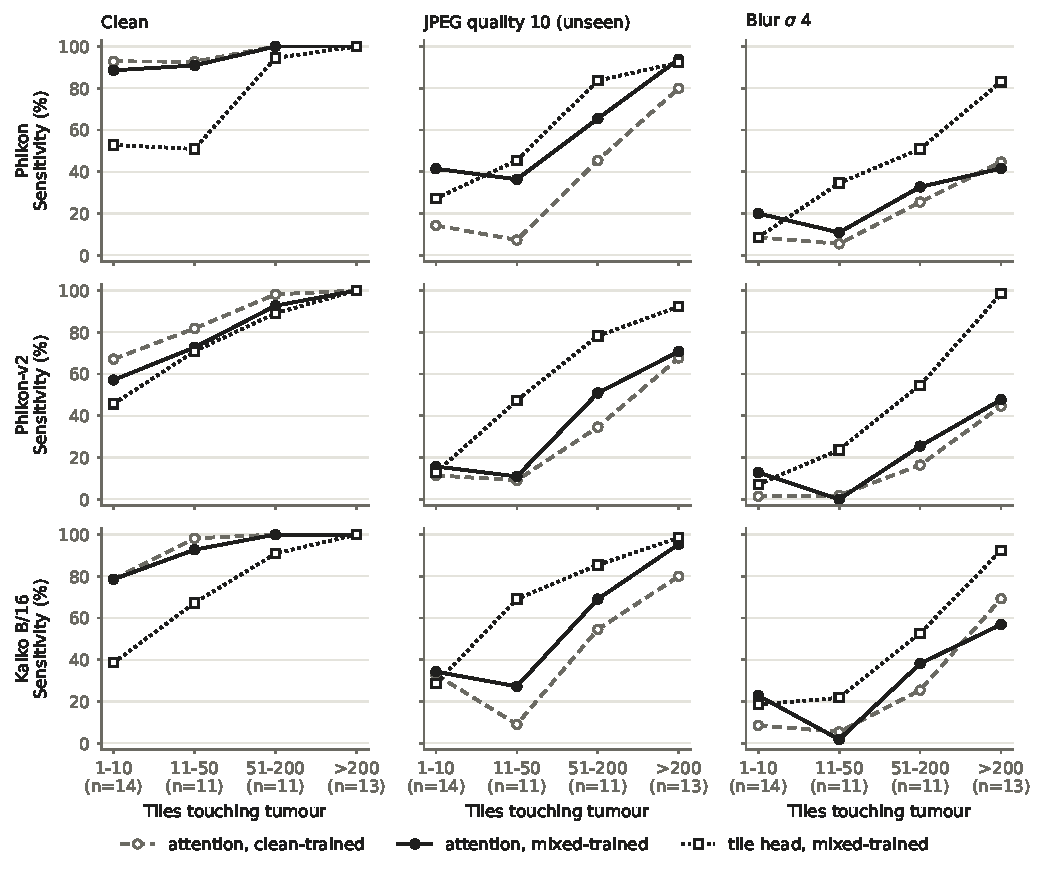
\includegraphics[width=\linewidth]{fig2_sensitivity_by_size.pdf}
\caption{Sensitivity at 95\% specificity by tumour size (number of 10x tiles touching tumour), for the three pathology encoders (rows) on clean slides, at JPEG quality 10 and at blur $\sigma$ 4 (columns). Mean of five seeds; $n$ is the number of test tumour slides in each size group.}
\label{fig:size}
\end{figure}

\subsection{Hospital and slide size}
\label{sec:hospital}

The test set is not balanced between centres: micrometastases are 11 RUMC and 16 UMCU slides, while normal slides are 50 and 30. Under blur $\sigma$ 4, the clean-trained attention scores of Phikon and Phikon-v2 tell the centres apart almost perfectly among normal slides (Table~\ref{tab:hospital}): Phikon gives normal UMCU slides lower scores than RUMC ones (AUC 2.5), Phikon-v2 higher (100.0). The same synthetic blur therefore shifts the two centres' slides differently, and the pooled AUC mixes this shift with the tumour signal. For Phikon-v2 the pooled micrometastasis AUC under blur is 50.0, while within each centre it is 36.5 and 22.8: the centre shift hides a below-chance result. Mixed training weakens the centre effect without removing it. Even on clean slides, Phikon's clean-trained scores separate the centres among normal slides (82.3), although within-centre AUC stays at 99.0 and 99.8.

Within each centre, micrometastasis slides still score below normal slides under blur $\sigma$ 4 for the clean-trained attention heads (AUC 22.8 to 47.1). We do not have an explanation for this.

Slide size is a second confound. Among normal slides, the tile head's score rises with the amount of tissue under JPEG (rank correlation 0.60 to 0.63 for the mixed-trained tile heads of the pathology encoders at quality 10), because more tiles give more chances of a high-scoring false positive. This is a known weakness of top-$k$ pooling and part of why the tile head detects fewer of the smallest metastases.

\begin{table}[h]\centering\small
\caption{Attention MIL by centre, on clean slides and at blur $\sigma$ 4. AUC in \%, mean of five seeds: tumour against normal slides within each centre; micrometastasis slides against normal slides within each centre; and how well the score separates UMCU from RUMC among normal slides (50 = not at all).}
\label{tab:hospital}
\setlength{\tabcolsep}{4pt}
\resizebox{\linewidth}{!}{\begin{tabular}{@{}llccccc@{}}
\toprule
Condition & Encoder, training & AUC RUMC & AUC UMCU & Micro RUMC & Micro UMCU & Centre from score\\
\midrule
Clean & Phikon, clean & 99.0 & 99.8 & 97.8 & 99.8 & 82.3\\
 & Phikon, mixed & 98.7 & 99.7 & 97.2 & 99.5 & 62.6\\
 & Kaiko B/16, clean & 98.2 & 99.2 & 96.1 & 98.7 & 57.6\\
 & Kaiko B/16, mixed & 98.6 & 99.4 & 97.1 & 99.0 & 47.7\\
 & Phikon-v2, clean & 96.0 & 98.0 & 92.0 & 96.9 & 46.6\\
 & Phikon-v2, mixed & 95.6 & 94.9 & 93.0 & 92.0 & 32.5\\
\addlinespace
Blur $\sigma$ 4 & Phikon, clean & 57.5 & 63.1 & 34.9 & 47.1 & 2.5\\
 & Phikon, mixed & 58.8 & 52.8 & 48.1 & 40.8 & 33.1\\
 & Kaiko B/16, clean & 60.7 & 51.5 & 40.3 & 32.0 & 28.5\\
 & Kaiko B/16, mixed & 64.3 & 58.6 & 54.8 & 41.5 & 36.6\\
 & Phikon-v2, clean & 51.6 & 45.1 & 36.5 & 22.8 & 100.0\\
 & Phikon-v2, mixed & 56.2 & 46.4 & 47.4 & 26.6 & 83.6\\
\bottomrule
\end{tabular}}
\end{table}

\section{Discussion}

\textbf{The first report's answer holds one level up, with a qualification.} For compression, most of what the slide pipeline loses is lost in the head: the frozen embeddings still separate tumour tiles, and a head trained on mixed tiles recovers much of the slide-level accuracy. The qualification is supervision. An attention head that learns only from slide labels has to discover about 50 tumour tiles among 2,000; when degradation moves tumour embeddings far from their clean position, as for Phikon-v2, mixed training does not teach it where to look. A head given tile labels does learn it. Encoders that drift most may therefore need tile-level supervision, or a different aggregator, to benefit from degradation-aware training.

\textbf{Which head is best depends on image quality.} On clean slides, attention beats the tile head by 3.4 to 7.5 AUC points for the pathology encoders and detects small metastases far better. Under JPEG quality 10 and blur $\sigma$ 4, the mixed-trained tile head is ahead of the mixed-trained attention head by 8 to 16 points. A comparison of aggregators on clean slides alone says little about how they behave on degraded ones, much as a comparison of encoders under a clean probe did in the first report.

\textbf{What slide-level robustness studies should report.} Pooled AUC on CAMELYON16 hides three things we found: the operating-point loss, its concentration in small metastases, and centre effects that can hide or invert a result. We suggest reporting sensitivity at a fixed specificity, broken down by tumour size, and AUC within each centre.

\textbf{What this means for a laboratory.} If compressed slides are expected, degraded examples should be included when the slide head is trained, and the head's ability to find small lesions should be checked on degraded data specifically. Heavy blur at 10x cannot be fixed by the head for small metastases; the remedy is at acquisition or at higher magnification.

\section{Limitations}

\begin{itemize}
\item \textbf{One test set.} 129 slides, 49 with tumour, from two centres. Intervals for macro- and micrometastasis subsets are wide.
\item \textbf{10x only.} Tiles are at 0.91 to 0.97 microns per pixel. Results on small metastases, and on blur, may differ at 20x or 40x.
\item \textbf{Synthetic degradations, applied per tile.} Blur and JPEG are not calibrated to a scanner, and the same level is a different perturbation for the two centres' images, as Section~\ref{sec:hospital} shows.
\item \textbf{Post hoc analyses.} The tile head and the analyses in Sections~\ref{sec:encoder} to~\ref{sec:hospital} were designed after the first results. Their settings were fixed before they were run and not tuned on the test set, but they were chosen to explain results already seen.
\item \textbf{The tile head is not a fair competitor.} It uses the lesion annotations, which the attention head does not. It is a diagnostic of where the signal is.
\item \textbf{One configuration per head and one draw of mixed tiles.} The attention head's settings were fixed in advance and not tuned; each training tile has one fixed degraded version.
\item \textbf{Thresholds from the test set.} Sensitivity at 95\% specificity uses a threshold set on the test normal slides, as is usual for this measure; it is not a deployable threshold.
\item \textbf{Annotations.} Twenty training tumour slides are not exhaustively annotated, which affects only the tile head and probe, whose normal tiles come from normal slides.
\item \textbf{Four encoders.} Larger and more recent encoders were not accessible to us.
\item \textbf{Not peer reviewed.} This is a technical report by a single author.
\end{itemize}

\sloppy
\section*{Code and data availability}

Code, the slide manifest, per-slide test predictions for every encoder, head, training set, seed and condition, and all result tables are at \url{https://github.com/dinakar0745/camelyon-slide-study} under the MIT licence. The figures and tables in this report are generated from those results by \texttt{paper/make\_paper.py}. CAMELYON16 is available from the Registry of Open Data on AWS.

\section*{Licences of models and data}

Phikon and Phikon-v2 are released by Owkin under a non-commercial licence, and the Kaiko ViT-B/16 weights under a non-commercial licence. DINOv2 is released under Apache 2.0. CAMELYON16 is released under CC0. This work is non-commercial research.

\section*{Funding and competing interests}

This work received no funding. The author declares no competing interests.

\section*{Use of AI assistance}

Claude (Anthropic), an AI assistant, was used to help write the pipeline and analysis code, to search the related literature, and to draft and edit the text of this report. The author ran all experiments and takes responsibility for the content.

\section*{References}

\begin{list}{}{\setlength{\leftmargin}{1.5em}\setlength{\itemindent}{-1.5em}\setlength{\itemsep}{0.25em}\setlength{\parsep}{0pt}}\small\raggedright
\item Aben N, de Jong ED, Gatopoulos I, K\"anzig N, Karasikov M, Lagr\'e A, Moser R, van Doorn J, Tang F (2024). Towards Large-Scale Training of Pathology Foundation Models. arXiv:2404.15217.
\item Campanella G, Hanna MG, Geneslaw L, Miraflor A, Werneck Krauss Silva V, Busam KJ, Brogi E, Reuter VE, Klimstra DS, Fuchs TJ (2019). Clinical-grade computational pathology using weakly supervised deep learning on whole slide images. Nature Medicine 25(8), 1301--1309.
\item de Jong ED, Marcus E, Teuwen J (2025). Current Pathology Foundation Models are unrobust to Medical Center Differences. arXiv:2501.18055.
\item Ehteshami Bejnordi B, Veta M, van Diest PJ, van Ginneken B, Karssemeijer N, Litjens G, van der Laak JAWM, and the CAMELYON16 Consortium (2017). Diagnostic Assessment of Deep Learning Algorithms for Detection of Lymph Node Metastases in Women With Breast Cancer. JAMA 318(22), 2199--2210.
\item Filiot A, Ghermi R, Olivier A, Jacob P, Fidon L, Mac Kain A, Saillard C, Schiratti J-B (2023). Scaling Self-Supervised Learning for Histopathology with Masked Image Modeling. medRxiv, doi:10.1101/2023.07.21.23292757.
\item Filiot A, Jacob P, Mac Kain A, Saillard C (2024). Phikon-v2, A large and public feature extractor for biomarker prediction. arXiv:2409.09173.
\item Hasan M, Faruk MO, El-Sakka MR (2026). Compression-Induced Representation Drift in Pathology Foundation Models. Electronics 15(18), 4186.
\item Ilse M, Tomczak JM, Welling M (2018). Attention-based Deep Multiple Instance Learning. Proceedings of the 35th International Conference on Machine Learning, PMLR 80, 2127--2136.
\item K\"omen J, de Jong ED, Hense J, Marienwald H, Dippel J, Naumann P, Marcus E, Ruff L, Alber M, Teuwen J, Klauschen F, M\"uller K-R (2026). Towards robust foundation models for digital pathology. Nature Communications 17, 5218. doi:10.1038/s41467-026-73923-2.
\item Litjens G, Bandi P, Ehteshami Bejnordi B, Geessink O, Balkenhol M, Bult P, Halilovic A, Hermsen M, van de Loo R, Vogels R, Manson QF, Stathonikos N, Baidoshvili A, van Diest P, Wauters C, van Dijk M, van der Laak J (2018). 1399 H\&E-stained sentinel lymph node sections of breast cancer patients: the CAMELYON dataset. GigaScience 7(6), giy065. doi:10.1093/gigascience/giy065.
\item Oquab M, Darcet T, Moutakanni T, Vo H, Szafraniec M, Khalidov V, Fernandez P, Haziza D, Massa F, El-Nouby A, Assran M, Ballas N, Galuba W, Howes R, Huang P-Y, Li S-W, Misra I, Rabbat M, Sharma V, Synnaeve G, Xu H, Jegou H, Mairal J, Labatut P, Joulin A, Bojanowski P (2023). DINOv2: Learning Robust Visual Features without Supervision. arXiv:2304.07193.
\item Pathakota D (2026). Is It the Encoder or the Probe? Acquisition-Artifact Robustness of Pathology Foundation Models. Technical report, Zenodo, doi:10.5281/zenodo.23162508.
\item Yajnik D, Asif A, Minhas F (2026). The Good, the Bad, and the Brittle: Benchmarking Robustness and Generalisation of Histopathology Foundation Models. arXiv:2607.04401.
\end{list}

\clearpage
\appendix
\section*{Appendix: full results}

\renewcommand{\topfraction}{0.95}\renewcommand{\textfraction}{0.02}\renewcommand{\floatpagefraction}{0.9}

\begin{table}[H]\centering\small
\caption{Gain from mixed training in AUC points, mean over five seeds with 95\% bootstrap interval, on all test slides and on macro- and micrometastasis slides against all normal slides. Bold intervals exclude zero.}
\label{tab:gains}
\setlength{\tabcolsep}{3pt}
\resizebox{\linewidth}{!}{\begin{tabular}{@{}llcccc@{}}
\toprule
Head & Slides & Phikon & Kaiko B/16 & Phikon-v2 & DINOv2-L\\
\midrule
Attention MIL, JPEG Q15 & all & \textbf{+12.2 {\scriptsize[+5.9, +18.8]}} & \textbf{+14.4 {\scriptsize[+8.4, +20.6]}} & +2.3 {\scriptsize[-2.6, +7.2]} & \textbf{+4.1 {\scriptsize[+0.1, +8.3]}}\\
 & macro & \textbf{+10.8 {\scriptsize[+2.5, +21.3]}} & \textbf{+5.0 {\scriptsize[+0.7, +10.8]}} & -0.1 {\scriptsize[-5.5, +4.3]} & \textbf{+1.9 {\scriptsize[+0.2, +4.5]}}\\
 & micro & \textbf{+13.4 {\scriptsize[+5.2, +22.4]}} & \textbf{+22.1 {\scriptsize[+13.3, +31.5]}} & +4.3 {\scriptsize[-3.5, +11.9]} & +5.9 {\scriptsize[-0.9, +12.7]}\\
\addlinespace
Attention MIL, JPEG Q10 (unseen) & all & \textbf{+16.7 {\scriptsize[+9.1, +24.1]}} & \textbf{+13.2 {\scriptsize[+7.8, +18.8]}} & -0.3 {\scriptsize[-5.0, +4.5]} & +4.3 {\scriptsize[-0.1, +8.6]}\\
 & macro & \textbf{+11.7 {\scriptsize[+3.5, +21.3]}} & \textbf{+6.8 {\scriptsize[+2.1, +12.6]}} & -1.2 {\scriptsize[-6.0, +3.2]} & \textbf{+3.2 {\scriptsize[+0.3, +7.5]}}\\
 & micro & \textbf{+20.7 {\scriptsize[+10.0, +31.5]}} & \textbf{+18.3 {\scriptsize[+10.4, +26.7]}} & +0.5 {\scriptsize[-6.4, +7.7]} & +5.2 {\scriptsize[-1.2, +11.8]}\\
\addlinespace
Attention MIL, Blur $\sigma$ 4 & all & +2.9 {\scriptsize[-4.4, +10.3]} & +4.4 {\scriptsize[-1.3, +10.2]} & -1.4 {\scriptsize[-8.6, +6.2]} & \textbf{+5.9 {\scriptsize[+1.2, +10.8]}}\\
 & macro & -1.3 {\scriptsize[-11.5, +9.2]} & -2.1 {\scriptsize[-9.8, +5.3]} & +3.9 {\scriptsize[-4.6, +12.9]} & \textbf{+10.8 {\scriptsize[+4.6, +17.5]}}\\
 & micro & +6.3 {\scriptsize[-2.4, +15.0]} & \textbf{+9.6 {\scriptsize[+2.0, +16.9]}} & -5.7 {\scriptsize[-16.0, +4.6]} & +1.9 {\scriptsize[-3.7, +8.0]}\\
\addlinespace
Tile head, JPEG Q15 & all & \textbf{+13.5 {\scriptsize[+6.5, +20.9]}} & +1.8 {\scriptsize[-2.4, +6.0]} & \textbf{+7.3 {\scriptsize[+1.3, +13.3]}} & -1.4 {\scriptsize[-6.7, +3.4]}\\
 & macro & +4.7 {\scriptsize[-0.8, +13.1]} & \textbf{+3.9 {\scriptsize[+0.1, +9.0]}} & \textbf{+7.1 {\scriptsize[+1.5, +13.8]}} & +1.0 {\scriptsize[-1.6, +3.3]}\\
 & micro & \textbf{+20.7 {\scriptsize[+10.1, +30.9]}} & +0.1 {\scriptsize[-6.2, +6.0]} & +7.6 {\scriptsize[-1.6, +16.4]} & -3.3 {\scriptsize[-12.0, +5.0]}\\
\addlinespace
Tile head, JPEG Q10 (unseen) & all & \textbf{+17.3 {\scriptsize[+8.0, +26.8]}} & \textbf{+7.5 {\scriptsize[+2.9, +12.4]}} & +6.0 {\scriptsize[-1.5, +14.1]} & -0.3 {\scriptsize[-6.1, +5.3]}\\
 & macro & +4.7 {\scriptsize[-0.9, +13.9]} & \textbf{+6.7 {\scriptsize[+2.0, +12.6]}} & \textbf{+9.5 {\scriptsize[+1.8, +19.6]}} & \textbf{+4.9 {\scriptsize[+0.8, +10.4]}}\\
 & micro & \textbf{+27.5 {\scriptsize[+14.5, +40.5]}} & \textbf{+8.2 {\scriptsize[+1.2, +15.8]}} & +3.1 {\scriptsize[-7.0, +13.7]} & -4.5 {\scriptsize[-12.9, +4.3]}\\
\addlinespace
Tile head, Blur $\sigma$ 4 & all & +10.4 {\scriptsize[-1.0, +21.3]} & \textbf{+18.4 {\scriptsize[+6.9, +29.5]}} & \textbf{+11.6 {\scriptsize[+0.8, +22.2]}} & +5.1 {\scriptsize[-2.1, +12.1]}\\
 & macro & \textbf{+20.8 {\scriptsize[+8.7, +33.1]}} & \textbf{+28.1 {\scriptsize[+16.8, +39.4]}} & \textbf{+30.2 {\scriptsize[+20.4, +41.3]}} & \textbf{+16.7 {\scriptsize[+8.6, +24.9]}}\\
 & micro & +2.0 {\scriptsize[-12.3, +16.3]} & +10.4 {\scriptsize[-5.3, +27.4]} & -3.6 {\scriptsize[-17.7, +10.9]} & -4.3 {\scriptsize[-12.6, +3.9]}\\
\bottomrule
\end{tabular}}
\end{table}

\begin{table}[H]\centering\small
\caption{Mean pooling. Slide AUC in \%, all 129 test slides, mean $\pm$ standard deviation over five seeds, for heads trained on clean (C) and mixed (M) embeddings. JPEG Q10 was not in the mixed training set.}
\label{tab:app-mean}
\setlength{\tabcolsep}{3.5pt}
\begin{tabular}{lrrrrrrrr}
\toprule
 & \multicolumn{2}{c}{Phikon} & \multicolumn{2}{c}{Kaiko B/16} & \multicolumn{2}{c}{Phikon-v2} & \multicolumn{2}{c}{DINOv2-L}\\
\cmidrule(lr){2-3}\cmidrule(lr){4-5}\cmidrule(lr){6-7}\cmidrule(lr){8-9}
Condition & C & M & C & M & C & M & C & M\\
\midrule
Clean & 66.5{\scriptsize$\pm$3.1} & 67.1{\scriptsize$\pm$2.9} & 64.3{\scriptsize$\pm$2.3} & 66.5{\scriptsize$\pm$2.1} & 61.3{\scriptsize$\pm$3.8} & 65.2{\scriptsize$\pm$2.4} & 59.2{\scriptsize$\pm$0.6} & 58.1{\scriptsize$\pm$4.0}\\
Blur $\sigma$ 2 & 63.7{\scriptsize$\pm$3.4} & 68.1{\scriptsize$\pm$1.4} & 66.7{\scriptsize$\pm$2.2} & 69.7{\scriptsize$\pm$1.3} & 52.0{\scriptsize$\pm$2.8} & 53.9{\scriptsize$\pm$3.5} & 60.0{\scriptsize$\pm$3.7} & 60.9{\scriptsize$\pm$4.1}\\
Blur $\sigma$ 4 & 43.4{\scriptsize$\pm$6.7} & 45.9{\scriptsize$\pm$7.8} & 38.4{\scriptsize$\pm$0.8} & 39.9{\scriptsize$\pm$1.3} & 36.6{\scriptsize$\pm$3.4} & 39.2{\scriptsize$\pm$4.7} & 46.0{\scriptsize$\pm$7.1} & 48.7{\scriptsize$\pm$8.5}\\
JPEG Q30 & 62.2{\scriptsize$\pm$4.2} & 57.9{\scriptsize$\pm$3.0} & 62.2{\scriptsize$\pm$2.0} & 61.3{\scriptsize$\pm$1.6} & 61.3{\scriptsize$\pm$6.0} & 61.4{\scriptsize$\pm$4.0} & 55.9{\scriptsize$\pm$2.5} & 61.0{\scriptsize$\pm$4.9}\\
JPEG Q15 & 60.3{\scriptsize$\pm$3.2} & 60.3{\scriptsize$\pm$4.3} & 63.6{\scriptsize$\pm$3.1} & 62.3{\scriptsize$\pm$3.8} & 55.4{\scriptsize$\pm$6.2} & 56.8{\scriptsize$\pm$5.6} & 55.6{\scriptsize$\pm$4.3} & 62.1{\scriptsize$\pm$5.9}\\
JPEG Q10 & 53.2{\scriptsize$\pm$5.2} & 55.5{\scriptsize$\pm$5.3} & 63.9{\scriptsize$\pm$3.2} & 62.5{\scriptsize$\pm$4.5} & 55.1{\scriptsize$\pm$3.9} & 58.5{\scriptsize$\pm$4.6} & 52.7{\scriptsize$\pm$5.0} & 58.2{\scriptsize$\pm$7.9}\\
Stain $\alpha$ 0.3 & 67.0{\scriptsize$\pm$4.2} & 66.9{\scriptsize$\pm$2.6} & 66.4{\scriptsize$\pm$3.6} & 67.6{\scriptsize$\pm$3.8} & 57.1{\scriptsize$\pm$5.6} & 65.4{\scriptsize$\pm$4.4} & 56.5{\scriptsize$\pm$1.3} & 55.9{\scriptsize$\pm$6.2}\\
\bottomrule
\end{tabular}
\end{table}

\begin{table}[H]\centering\small
\caption{Max pooling. Slide AUC in \%, all 129 test slides, mean $\pm$ standard deviation over five seeds, for heads trained on clean (C) and mixed (M) embeddings. JPEG Q10 was not in the mixed training set.}
\label{tab:app-max}
\setlength{\tabcolsep}{3.5pt}
\begin{tabular}{lrrrrrrrr}
\toprule
 & \multicolumn{2}{c}{Phikon} & \multicolumn{2}{c}{Kaiko B/16} & \multicolumn{2}{c}{Phikon-v2} & \multicolumn{2}{c}{DINOv2-L}\\
\cmidrule(lr){2-3}\cmidrule(lr){4-5}\cmidrule(lr){6-7}\cmidrule(lr){8-9}
Condition & C & M & C & M & C & M & C & M\\
\midrule
Clean & 79.4{\scriptsize$\pm$1.6} & 81.0{\scriptsize$\pm$3.9} & 77.1{\scriptsize$\pm$2.2} & 74.9{\scriptsize$\pm$1.4} & 75.4{\scriptsize$\pm$1.3} & 75.2{\scriptsize$\pm$3.0} & 61.3{\scriptsize$\pm$2.7} & 63.3{\scriptsize$\pm$0.8}\\
Blur $\sigma$ 2 & 77.3{\scriptsize$\pm$1.9} & 78.2{\scriptsize$\pm$1.2} & 69.4{\scriptsize$\pm$0.7} & 69.3{\scriptsize$\pm$2.8} & 64.5{\scriptsize$\pm$3.6} & 60.0{\scriptsize$\pm$3.2} & 60.8{\scriptsize$\pm$0.9} & 65.7{\scriptsize$\pm$2.4}\\
Blur $\sigma$ 4 & 54.1{\scriptsize$\pm$3.5} & 57.0{\scriptsize$\pm$2.3} & 65.1{\scriptsize$\pm$4.3} & 61.8{\scriptsize$\pm$1.7} & 59.3{\scriptsize$\pm$1.9} & 59.4{\scriptsize$\pm$5.5} & 58.9{\scriptsize$\pm$4.0} & 63.3{\scriptsize$\pm$2.1}\\
JPEG Q30 & 69.3{\scriptsize$\pm$1.4} & 74.3{\scriptsize$\pm$1.5} & 73.2{\scriptsize$\pm$2.2} & 73.8{\scriptsize$\pm$0.9} & 65.9{\scriptsize$\pm$3.1} & 60.8{\scriptsize$\pm$4.5} & 58.0{\scriptsize$\pm$5.3} & 63.9{\scriptsize$\pm$1.9}\\
JPEG Q15 & 65.9{\scriptsize$\pm$2.3} & 71.0{\scriptsize$\pm$2.5} & 67.6{\scriptsize$\pm$4.2} & 73.3{\scriptsize$\pm$0.5} & 70.1{\scriptsize$\pm$2.2} & 69.3{\scriptsize$\pm$4.8} & 54.4{\scriptsize$\pm$5.9} & 63.3{\scriptsize$\pm$1.2}\\
JPEG Q10 & 61.8{\scriptsize$\pm$2.9} & 69.2{\scriptsize$\pm$4.3} & 65.2{\scriptsize$\pm$3.5} & 68.9{\scriptsize$\pm$1.3} & 65.6{\scriptsize$\pm$3.9} & 70.6{\scriptsize$\pm$4.5} & 57.7{\scriptsize$\pm$5.4} & 60.6{\scriptsize$\pm$4.7}\\
Stain $\alpha$ 0.3 & 79.3{\scriptsize$\pm$0.9} & 81.2{\scriptsize$\pm$5.3} & 78.5{\scriptsize$\pm$3.1} & 74.6{\scriptsize$\pm$1.2} & 73.2{\scriptsize$\pm$1.3} & 74.1{\scriptsize$\pm$4.0} & 59.1{\scriptsize$\pm$3.8} & 67.3{\scriptsize$\pm$1.0}\\
\bottomrule
\end{tabular}
\end{table}

\begin{table}[H]\centering\small
\caption{Attention MIL. Slide AUC in \%, all 129 test slides, mean $\pm$ standard deviation over five seeds, for heads trained on clean (C) and mixed (M) embeddings. JPEG Q10 was not in the mixed training set.}
\label{tab:app-abmil}
\setlength{\tabcolsep}{3.5pt}
\begin{tabular}{lrrrrrrrr}
\toprule
 & \multicolumn{2}{c}{Phikon} & \multicolumn{2}{c}{Kaiko B/16} & \multicolumn{2}{c}{Phikon-v2} & \multicolumn{2}{c}{DINOv2-L}\\
\cmidrule(lr){2-3}\cmidrule(lr){4-5}\cmidrule(lr){6-7}\cmidrule(lr){8-9}
Condition & C & M & C & M & C & M & C & M\\
\midrule
Clean & 98.9{\scriptsize$\pm$0.4} & 98.8{\scriptsize$\pm$0.4} & 98.6{\scriptsize$\pm$0.4} & 98.5{\scriptsize$\pm$0.2} & 96.4{\scriptsize$\pm$1.5} & 93.8{\scriptsize$\pm$0.4} & 77.3{\scriptsize$\pm$2.8} & 76.4{\scriptsize$\pm$2.3}\\
Blur $\sigma$ 2 & 90.1{\scriptsize$\pm$3.6} & 95.5{\scriptsize$\pm$1.0} & 97.6{\scriptsize$\pm$0.6} & 97.9{\scriptsize$\pm$0.3} & 86.1{\scriptsize$\pm$4.8} & 87.5{\scriptsize$\pm$2.1} & 71.0{\scriptsize$\pm$5.0} & 71.7{\scriptsize$\pm$1.8}\\
Blur $\sigma$ 4 & 51.0{\scriptsize$\pm$1.5} & 53.9{\scriptsize$\pm$5.4} & 55.6{\scriptsize$\pm$3.4} & 60.0{\scriptsize$\pm$2.6} & 56.2{\scriptsize$\pm$1.7} & 54.8{\scriptsize$\pm$2.9} & 53.0{\scriptsize$\pm$3.8} & 58.9{\scriptsize$\pm$5.7}\\
JPEG Q30 & 90.4{\scriptsize$\pm$1.0} & 92.3{\scriptsize$\pm$1.1} & 93.6{\scriptsize$\pm$1.1} & 96.7{\scriptsize$\pm$0.9} & 84.6{\scriptsize$\pm$4.4} & 85.7{\scriptsize$\pm$3.4} & 72.0{\scriptsize$\pm$4.6} & 76.3{\scriptsize$\pm$3.5}\\
JPEG Q15 & 74.0{\scriptsize$\pm$4.2} & 86.2{\scriptsize$\pm$2.5} & 75.3{\scriptsize$\pm$3.5} & 89.7{\scriptsize$\pm$3.9} & 72.7{\scriptsize$\pm$5.4} & 75.0{\scriptsize$\pm$2.2} & 70.5{\scriptsize$\pm$3.0} & 74.6{\scriptsize$\pm$2.4}\\
JPEG Q10 & 63.1{\scriptsize$\pm$4.1} & 79.7{\scriptsize$\pm$4.5} & 67.9{\scriptsize$\pm$3.0} & 81.1{\scriptsize$\pm$6.3} & 68.1{\scriptsize$\pm$4.3} & 67.8{\scriptsize$\pm$3.7} & 70.0{\scriptsize$\pm$2.8} & 74.4{\scriptsize$\pm$2.5}\\
Stain $\alpha$ 0.3 & 99.4{\scriptsize$\pm$0.1} & 99.2{\scriptsize$\pm$0.2} & 98.5{\scriptsize$\pm$0.3} & 98.2{\scriptsize$\pm$0.4} & 97.2{\scriptsize$\pm$1.2} & 94.5{\scriptsize$\pm$1.3} & 77.9{\scriptsize$\pm$2.2} & 78.4{\scriptsize$\pm$2.4}\\
\bottomrule
\end{tabular}
\end{table}

\begin{table}[H]\centering\small
\caption{Tile head. Slide AUC in \%, all 129 test slides, mean $\pm$ standard deviation over five seeds, for heads trained on clean (C) and mixed (M) embeddings. JPEG Q10 was not in the mixed training set.}
\label{tab:app-tileprobe}
\setlength{\tabcolsep}{3.5pt}
\begin{tabular}{lrrrrrrrr}
\toprule
 & \multicolumn{2}{c}{Phikon} & \multicolumn{2}{c}{Kaiko B/16} & \multicolumn{2}{c}{Phikon-v2} & \multicolumn{2}{c}{DINOv2-L}\\
\cmidrule(lr){2-3}\cmidrule(lr){4-5}\cmidrule(lr){6-7}\cmidrule(lr){8-9}
Condition & C & M & C & M & C & M & C & M\\
\midrule
Clean & 92.7{\scriptsize$\pm$1.2} & 89.9{\scriptsize$\pm$1.1} & 91.1{\scriptsize$\pm$1.6} & 90.0{\scriptsize$\pm$0.9} & 93.0{\scriptsize$\pm$2.8} & 87.5{\scriptsize$\pm$1.0} & 78.8{\scriptsize$\pm$1.9} & 75.0{\scriptsize$\pm$2.5}\\
Blur $\sigma$ 2 & 73.2{\scriptsize$\pm$2.0} & 86.5{\scriptsize$\pm$1.2} & 83.4{\scriptsize$\pm$2.8} & 88.9{\scriptsize$\pm$1.7} & 77.8{\scriptsize$\pm$5.7} & 82.8{\scriptsize$\pm$1.2} & 72.3{\scriptsize$\pm$2.7} & 72.6{\scriptsize$\pm$2.6}\\
Blur $\sigma$ 4 & 59.3{\scriptsize$\pm$4.0} & 69.8{\scriptsize$\pm$1.2} & 52.4{\scriptsize$\pm$3.9} & 70.8{\scriptsize$\pm$1.4} & 58.0{\scriptsize$\pm$1.8} & 69.6{\scriptsize$\pm$0.9} & 53.9{\scriptsize$\pm$4.4} & 59.0{\scriptsize$\pm$1.5}\\
JPEG Q30 & 84.5{\scriptsize$\pm$2.8} & 90.2{\scriptsize$\pm$0.9} & 90.9{\scriptsize$\pm$0.8} & 91.2{\scriptsize$\pm$1.9} & 84.3{\scriptsize$\pm$5.0} & 86.2{\scriptsize$\pm$1.2} & 78.0{\scriptsize$\pm$1.1} & 75.8{\scriptsize$\pm$1.5}\\
JPEG Q15 & 74.4{\scriptsize$\pm$3.0} & 87.9{\scriptsize$\pm$0.8} & 87.5{\scriptsize$\pm$2.7} & 89.3{\scriptsize$\pm$2.0} & 77.7{\scriptsize$\pm$3.8} & 85.1{\scriptsize$\pm$0.7} & 78.2{\scriptsize$\pm$1.1} & 76.8{\scriptsize$\pm$3.0}\\
JPEG Q10 & 71.0{\scriptsize$\pm$1.5} & 88.2{\scriptsize$\pm$1.0} & 82.1{\scriptsize$\pm$2.7} & 89.6{\scriptsize$\pm$1.1} & 75.8{\scriptsize$\pm$1.9} & 81.9{\scriptsize$\pm$1.1} & 77.6{\scriptsize$\pm$0.4} & 77.3{\scriptsize$\pm$1.2}\\
Stain $\alpha$ 0.3 & 91.4{\scriptsize$\pm$1.8} & 91.9{\scriptsize$\pm$1.0} & 91.9{\scriptsize$\pm$1.6} & 89.4{\scriptsize$\pm$1.1} & 93.1{\scriptsize$\pm$2.1} & 88.6{\scriptsize$\pm$0.9} & 79.8{\scriptsize$\pm$2.6} & 80.4{\scriptsize$\pm$1.1}\\
\bottomrule
\end{tabular}
\end{table}


\end{document}
